Die wichtigsten Eigenschaften einer Beschreibungslogik sind
\emph{Ausdrucksstärke} und \emph{Komplexität}. Ausdruckstärke kann man
nicht linear quantifizieren, sondern nur beschreiben und
charakterisieren.

\subsection{Bisimulation}\label{bisimulation}

Bisimulation ist ein graphentheoretische Begriff, die ``Ähnlichkeit'' von Graphen beschreibt und eng mit der Ausdruckstärke von $\ALC$ zusammenhängt.

\begin{definition}{Bisimulation}

Seien $I_{1}$ und $I_{2}$ Interpretationen. Relation
$\rho \subseteq \Delta^{I_{1}} \times \Delta^{I_{2}}$ ist Bisimulation
zwischen $I_{1}$ und $I_{2}$, wenn gilt:

\begin{enumerate}
\def\labelenumi{\arabic{enumi}.}
\item
  Wenn $d_{1}\text{\ $\rho$}\text{\ d}_{2}$, dann gilt für alle
  Konzeptnamen A: $d_{1} \in A^{I_{1}}$ gdw. $d_{2} \in A^{I_{2}}$.
\item
  Wenn $d_{1}\text{\ $\rho$}\text{\ d}_{2}$ und
  $\left( d_{1},d_{1}^{'} \right) \in r^{I_{1}}$ für beliebigen
  Rollennamen $r$, dann gibt es ein $d_{2}^{'} \in \Delta^{I_{2}}$
  mit ${d'}_{1}\text{\ $\rho$}{\ d'}_{2}$ und
  $\left( d_{2},d_{2}^{'} \right) \in r^{I_{2}}$.
\item
  Wenn $d_{1}\text{\ $\rho$}\text{\ d}_{2}$ und
  $\left( d_{2},d_{2}^{'} \right) \in r^{I_{2}}$ für beliebigen
  Rollennamen $r$, dann gibt es ein $d_{1}^{'} \in \Delta^{I_{1}}$
  mit ${d'}_{1}\text{\ $\rho$}{\ d'}_{2}$ und
  $\left( d_{1},d_{1}^{'} \right) \in r^{I_{1}}$.
\end{enumerate}
\end{definition}

Seien $I_{1}$ und $I_{2}$ Interpretationen,
$d_{1} \in \Delta^{I_{1}}$, $d_{2} \in \Delta^{I_{2}}$:

$(I_{1},d_{1}) \sim (I_{2},d_{2})$: Es gibt Bisimulation $\rho$
zwischen $I_{1}$ und $I_{2}$ mit $d_{1}\text{\ $\rho$}\text{\ d}_{2}$.
Die leere Relation ist immer Bisimulation.

\begin{theorem}
Seien $I_{1}$, $I_{2}$ Interpretationen,
$d_{1} \in \Delta^{I_{1}}$ und $d_{2} \in \Delta^{I_{2}}$. Wenn
$(I_{1},d_{1}) \sim (I_{2},d_{2})$, dann gilt für alle ALC-Konzepte
$C$:

$$d_{1} \in C^{I_{1}}\ gdw.\ d_{2} \in C^{I_{2}}$$
\end{theorem}

\textbf{T3.2.}

\begin{proof}
Beweisskizze per Induktion über die Struktur von C. Sei $\rho$ eine
Bisimulation zwischen $I_{1}$ und $I_{2}$ mit
$d_{1}\text{\ $\rho$}\text{\ d}_{2}$.

\textbf{I.A.} $C = A$ ist Konzeptname. Nach Bedingung 1. der
Bisimulation gilt $$d_{1} \in A^{I_{1}}\ gdw.\ d_{2} \in A^{I_{2}}$$.

\textbf{I.S.} Unterscheide Fälle gemäß des äußersten Konstruktes von C.
Es genügen $\neg$,$\sqcap$, $\exists\text{r.C}$:

\begin{enumerate}
\def\labelenumi{\arabic{enumi}.}
\item
  $C = \neg D$
\end{enumerate}

\begin{quote}
\begin{equation}
\begin{split}
d_{1} \in C^{I_{1}} &\stackrel{Sem.}{gdw.} d_{1} \notin D^{\MI_{1}}\\
&\stackrel{I.V.}{gdw.} d_{2} \notin D^{\MI_{2}} \\
&\stackrel{Sem.}{gdw.} d_{2} \in C^{\MI_{2}}
\end{split}
\end{equation}
\end{quote}

\begin{enumerate}
\def\labelenumi{\arabic{enumi}.}
\item
  $C = D_{1} \sqcap D_{2}$
\end{enumerate}

\begin{quote}
\begin{equation}
\begin{split}
d_{1} \in C^{\MI_{1}} &\stackrel{Sem.}{gdw.} d_{1} \in D_{1}^{\MI_{1}}\ und\ d_{1} \in D_{2}^{\MI_{1}}\\
&\stackrel{I.V.}{gdw.} d_{2} \in D_{1}^{\MI_{2}}\ und\ d_{2} \in D_{2}^{\MI_{2}} \\
&\stackrel{Sem.}{gdw.} d_{2} \in C^{\MI_{2}}
\end{split}
\end{equation}
\end{quote}

\begin{enumerate}
\def\labelenumi{\arabic{enumi}.}
\item
  $C = \exists r.D$
\end{enumerate}

\begin{quote}
\begin{equation}
\begin{split}
d_{1} \in C^{\MI_{1}} &\stackrel{Sem.}{\Rightarrow} \exists e_1 : (d_1,e_1) \in r^{\MI_1}\ und\ e \in D^{\MI_1}\\
&\stackrel{2.Bed.}{\Rightarrow} \exists e_2 \in \Delta_2^{\MI_2}: (d_2,e_e) \in r^{\MI_2}\ und\ (e_1 \rho e_2) \\
&\stackrel{I.V.}{\Rightarrow} e_2 \in D^{\MI_2} \\
&\stackrel{Sem.}{\Rightarrow} d_{2} \in (\exists r.D)^{\MI_2} \\
&\stackrel{Sem.}{gdw.} d_2 \in C^{\MI_{2}}
\end{split}
\end{equation}
Rückrichtung analog, nur mit der 3. Bedingung.
\end{quote}
\end{proof}

\subsection{Ausdrucksstärke}\label{ausdrucksstuxe4rke}

\begin{definition}{Eigenschaft, Ausdrückbarkeit}

Eine \emph{Eigenschaft} $E$ ist eine Menge von Paaren $(\MI,d)$, wobei
$\MI$ eine Interpretation und $d \in \Delta^{\MI}$ ein Element in $\MI$ ist.

$E$ ist \emph{ausdrückbar in $\ALC$}, wenn es ein $\ALC$-Konzept $C$
gibt, so dass für alle $\MI$ und $d \in \Delta^{\MI}$ gilt:
$$\left( \MI,\ d \right) \in E\ gdw.\ d \in C^{\MI}$$
\end{definition}

\subsubsection{Anwendungen von Bisimulation I}\label{theorem-3.4}

\begin{theorem}
In $\ALC$ ist nicht ausdrückbar: 
\begin{itemize}
\item das $\ALCI$-Konzept $\exists r^{-}.\top$ 
\item die $\ALCQ$-Konzepte
\begin{itemize}
  \item $(\leq\ n\ r\ \top)$ für alle $n\ > 0$ und
  \item $(\geq\ n\ r\ \top)$ für alle $n\ > 1$
\end{itemize}
\end{itemize}
\end{theorem}

\textbf{T.3.3.}

Beweisskizze. Finde Bisimulation für die dies nicht gilt.

\begin{proof}
\textbf{$\exists r.\top$}

Betrachte 2 Interpretationen $\MI$ und $\MJ$

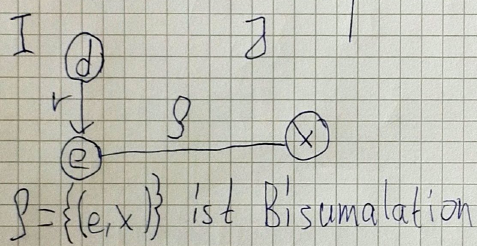
\includegraphics[width=3.71910in,height=1.83200in]{media/33inv.png}

Angenommen, es gäbe ein $\ALC$-Konzept $C$ mit $C \equiv \exists r^{-}.\top$. Dann gilt $e \in C^{\MI}$. Mit Theorem 3.2 folgt $x \in C^{\MJ}$, also hat x auch einen r-Vorgänger in $\MJ$. $\lightning$
\end{proof} 

\begin{proof}
$\leq\ n\ r\ \top$

Betrachte 2 Interpretationen $\MI$ und $\MJ$

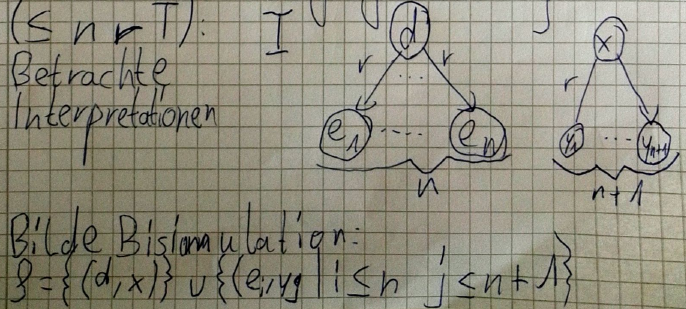
\includegraphics[width=3.71910in,height=1.83200in]{media/33low.png}

Angenommen, es gäbe ein $\ALC$-Konzept $C$ mit $C \equiv (\leq\ n\ r\ \top)$. Dann gilt $d \in C^{\MI}$. Mit Theorem 3.2 folgt $x \in C^{\MJ}$, also $x \in (\leq\ n\ r\ \top)$. $\lightning$
\end{proof}

Man sieht, dass die Argumentation zum Beweis der Nicht-Ausdrückbarkeit immer auf dasselbe hinausläuft:
\begin{theorem}

Sei $E$ eine Eigenschaft. Wenn es Interpretation $I_{1}$, $I_{2}$
und Elemente $d_{1} \in \Delta^{I_{1}}$ und
$d_{2} \in \Delta^{I_{2}}$ gibt, so dass

\begin{itemize}
\item
  $\left( I_{1},d_{1} \right) \in E$ und
  $\left( I_{2},d_{2} \right) \in E$ sowie
\item
  $(I_{1},d_{1}) \sim (I_{2},d_{2})$
\end{itemize}

dann ist $E$ nicht in $\ALC$ ausdrückbar.
\end{theorem}

\subsubsection{Anwendungen von Bisimulation II}\label{theorem-3.6}

Interpretation ist \emph{Baum} gdw. $(\Delta^{\MI}, \cdot^{\MI})$ Baum (endl. oder unendl.). $\ALC$ hat die \emph{Baummodelleigenschaft}

\begin{theorem}
Wenn ein ALC-Konzept $C$ bzgl. einer ALC-TBox $\MT$ erfüllbar ist,
dann haben $C$ und $\MT$ ein \underline{gemeinsames Baummodell} $\MI$. (mit $\MI$ Baum, Wurzel in $C^{\MI}$.)
\end{theorem}

\subsubsection{Unravelling}\label{unravelling}

Sei $\MI$ eine Interpretation und $d \in \Delta^{\MI}$. 

$d$-Pfad in $\MI$: Sequenz $d_{0}d_{1}\ldots d_{n - 1}$, $n > 0$ mit

\begin{itemize}
\item
  $d_{0} = d$
\item
  für alle $i < n$: es gibt Rollenname $r$ mit
  $\left( d_{i},d_{i + 1} \right) \in r^{\MI}$.
\end{itemize}

Wir setzen
$\text{end}\left( d_{0}\ldots d_{n - 1} \right) = d_{n - 1}$.

\begin{definition}{Unravelling}

Unravelling von $\MI$ an Stelle $d$ ist folgende Interpretation $\MJ$:

\begin{itemize}
\item
  $\Delta^{\MJ} =$ Menge aller $d$-Pfade in $\MI$
\item
  $A^{\MJ} = \left\{ p \in \Delta^{\MJ}\  \right|\text{\ end}\left( p \right) \in A^{\MI}\}$
\item
  $r^{\MJ} = \left\{ \left( p,p' \right) \in \Delta^{\MJ} \times \Delta^{\MJ}\ |\ \exists e:p^{'} = p \cdot e\ \mathrm{\text{und}}\ \left( \text{end}\left( p \right),e \right) \in r^{\MI} \right\}$
\end{itemize}

für alle Konzeptnamen $A$ und Rollennamne $r$
\end{definition}

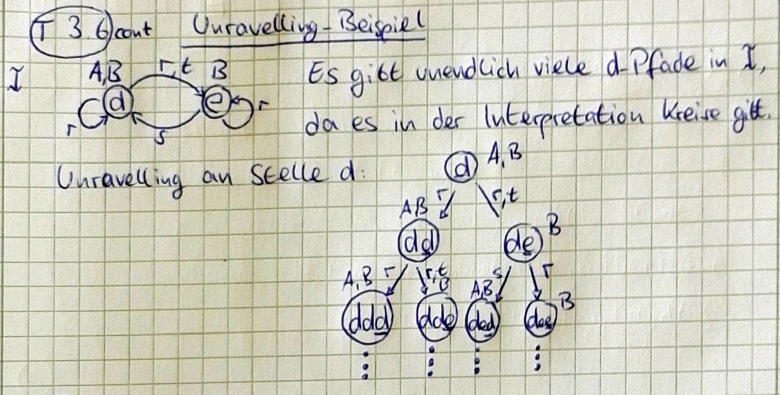
\includegraphics[width=4.71910in,height=1.83200in]{media/36unraveling.png}

Erklärung: Erzeuge Knoten, die den Folgen entsprechen, füge sie den
Konzepten hinzu, die als letztes Element in der Folge vorkommen und
erzeuge Kanten die den weiterführenden Rollen entsprechen.

\begin{lemma}\label{lemma37}
Sei $\MJ$ Unravelling von $\MI$ an Stelle $d$. Für alle $\ALC$-Konzepte $C$ und alle $p \in \Delta^{\MJ}$ gilt:
$$\text{end}\left( p \right) \in C^{\MI}\ gdw.\ p \in C^{\MJ}$$
\end{lemma}

\textbf{T3.7}

\begin{proof}
Mit Theorem genügt es folgende Bisimulation zu zeigen:
$$\left( I,end\left( p \right) \right)\sim\left( J,p \right)$$ Definiere Relation: $$\rho = \left\{ \left( \text{end}\left( p \right),p \right) \in \Delta^{\MI} \times \Delta^{\MJ}\  \right|\text{\ p\ }\mathrm{\text{ist}}\text{\ d}\mathrm{- Pfad}\}\ $$(Bilde
alle Knoten in $\MJ$ auf ihr Ende ab). 

Zur Bisimulation:

\begin{enumerate}
\def\labelenumi{\arabic{enumi}.}
\item
  gilt per Definition von $\MJ$.
\item
  Angenommen $e$ $\rho$ $p$ und
  $\left( e,e^{'} \right) \in r^{\MI}$. Dann $e = end\left( p \right)$
  per Konstruktion von $\MJ$. Wegen $\left( e,e^{'} \right) \in r^{\MI}$
  ist $pe'$ Pfad. Nach Konstruktion von $\MJ$ gilt
  $\left( p,pe^{'} \right) \in r^{\MJ}$.
\end{enumerate}
\end{proof}

Nun folgt Theorem 3.6.:

\textbf{Theorem 3.6} Wenn ein $\ALC$-Konzept $C$ bzgl. einer TBox $\MT$ erfüllbar ist, dann haben $C$ und $\MT$ ein gemeinsames Baummodell $\MI$.

\textbf{T3.8}
\begin{proof}
Sei $C$ erfüllbar bezüglich $\MT$. Dann gibt es Modell $\MI$ von $C$ und $\MT$. Sei $\MJ$ das Unravelling von $\MI$ an der Stelle
$d_0 \in C^{\MI}$.

Mit \hyperlink{lemma37}{Lemma 3.8} ist die Wurzel $d_0$ von $\MJ$ in $C^{\MJ}$. Noch zu zeigen: $\MJ$ ist Modell von $\MT$. 

Sei $D \sqsubseteq E$ in $\MT$ und $p \in D^{\MJ}$. Nach \protect\hyperlink{lemma37}{Lemma 3.8} ist dann $\text{end}\left( p \right) \in D^{\MI}$ und weil $\MI$ Modell von $\MT$ folgt $\text{end}\left( p \right) \in E^{\MI}$. Mit \protect\hyperlink{lemma37}{Lemma 3.8} folgt $p \in E^{\MJ} \Rightarrow J \vDash D \sqsubseteq E$.
\end{proof}

\subsubsection{Bisimulation versus Ausdrucksstärke}\label{bisimulation-versus-ausdrucksstuxe4rke}

Bisimulation entspricht nicht der Ausdrucksstärke von $\ALC$, denn die Gegenrichtung von Theorem 3.2 gilt nicht:

Es gibt Interpreatationen $\MI$ und $\MJ$ und $d \in \MI$, $x \in \MJ$, so dass $d \in C^{\MI}$ gdw. $x \in C^{\MJ}$ für alle $\ALC$-Konzepte $C$, aber $(\MI,d) \not\sim (\MJ,x)$. 

Beispiel:

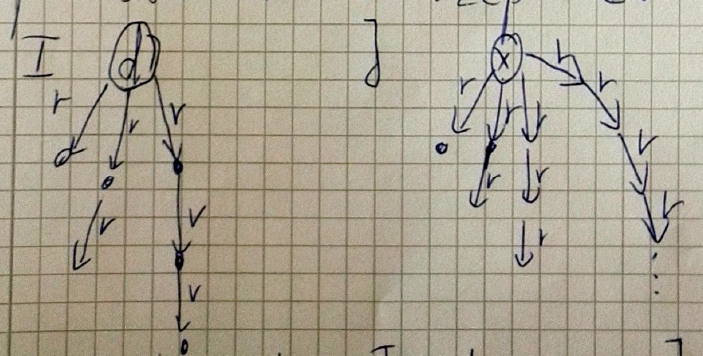
\includegraphics[width=3.71910in,height=1.83200in]{media/39bis.png}

Es gilt:

\begin{itemize}
  \item $d \in C^{\MI}$ gdw. $x \in C^{\MJ}$, falls ALC-Konzept C
  \item $(\MI,d) \not\sim (\MJ,x)$: für $y$ in $\MJ$ gibt es kein adäquates Element $e \in \Delta^{\MI}$ mit $e\ \rho\ y$
\end{itemize}

Sie gilt allerdings für verschiedene Klassen von Interpretationen, wie die Klasse aller endlichen Interpretationen oder die Klasse aller Interpretationen mit endlicher Verweigungszahl.

\subsubsection{Bisimulation für Erweiterungen von $\ALCI$}\label{bisimulation-in-alci}

Für $\ALCI$, $\ALCQ$ und $\ALCQI$ gibt es ebenfalls Bisimulationsbegriffe.

Fpr $\ALCI$ füge 2 Regeln hinzu, sodass Vorgänger auch simuliert sein müssen.

So kann man zudem zeigen, dass $\ALCI$, $\ALCQ$ und $\ALCQI$ die Baummodelleigenschaft haben.

\subsection{Ausdrucksstärke und
Modellkonstruktion}\label{ausdrucksstuxe4rke-und-modellkonstruktion}

In diesem Kapitel wird die endliche Modelleigenschaft und Filtration eingeführt.

\subsubsection{Größe von Konzepten und
TBoxen}\label{gruxf6uxdfe-von-konzepten-und-tboxen}

\begin{definition}{Größe}
\emph{Größe} $\left| C \right|$ eines ALC-Konzeptes $C$ ist induktiv
definiert:

\begin{itemize}
\item
  $\left| A \right| = 1$
\item
  $\left| \neg C \right| = \left| C \right| + 1$
\item
  $\left| C \sqcap D \right| = \left| C \sqcup D \right| = \left| C \right| + \left| D \right| + 1$
\item
  $\left| \exists r.C \right| = \left| \forall r.C \right| = \left| C \right| + 3$
\end{itemize}

\emph{Größe} $\left| C \right|$ einer TBox $\MT$ ist

\begin{itemize}
\item
  $\sum_{C \sqsubseteq D \in T}^{}{\left| C \right| + \left| D \right| + 1}$
\end{itemize}
\end{definition}

Intuitiv entspricht dies der Anzahl von Symbolen in $C$ bzw. $\MT$.

\subsubsection{Endliche/beschränkte Modelleigenschaft}

$\ALC$ hat \emph{endliche Modelleigenschaft}:

\begin{theorem}
Wenn ein $\ALC$-Konzept $C$ bzgl. einer $\ALC$-TBox $\MT$ erfüllbar ist, dann haben $C$ und $\MT$ ein gemeinsames \emph{endliches} Modell.
\end{theorem}

$\ALC$ hat sogar \emph{beschränkte Modelleigenschaft}:

\begin{theorem}
Wenn ein $\ALC$-Konzept $C$ bzgl. einer $\ALC$-TBox $\MT$ erfüllbar ist, dann haben $C$ und $\MT$ ein gemeinsames Modell der \emph{Kardinalität} $\leq 2^{|C|+|T|}$
\end{theorem}

\subsubsection{Typ}

Im Folgenden sei $C$ $\ALC$-Konzept und $\MT$ TBox, so dass $C$ erfüllbar bzgl. $\MT$.

Wir definieren den Begriff eines Typs:

\begin{itemize}
  \item ist Menge von Konzepten
  \item beschreibt einen Punkt $d \in \Delta^{\MI}$ in einer Interpreatation $\MI$
  \item Einschränkung auf Teilkonzepte von $C$ und $\MT$ (um Endlichkeit zu erreichen)
\end{itemize}

\subsubsection{Typ}\label{typ}

\begin{definition}{Teilkonzepte}
\begin{itemize}
\item
  $\text{sub}\left( C \right)$ ist Menge der Teilkonzepte von $C$
  (einschließlich $C$)
\item
  $\text{sub}\left( \MT \right) := \bigcup_{C \sqsubseteq D \in \MT}^{}{\text{sub}\left( C \right) \cup sub\left( D \right)}$
\item
  $\text{sub}\left( C,\MT \right) := sub\left( C \right) \cup sub\left( \MT \right)$
\end{itemize}
\end{definition}

\textbf{T3.10}

Beispiele: $$sub(\forall r.\exists r.(A \sqcap B)) = \{A,B,A \sqcap B, \exists r.(A \sqcap B), \forall r.\exists r.(A \sqcap B)\}$$
$$sub(\{A \sqsubseteq r.B, \forall r.B \sqsubseteq A\}) = \{A,B, \exists r.B, \forall r.B\}$$

\begin{lemma}

$\left| \text{sub}\left( C,T \right) \right| \leq \left| C \right| + \left| T \right|$
\end{lemma}

\begin{definition}{Typ von $d$}

Sei $\MI$ eine Interpretation, $d \in \Delta^{\MI}$. Der \emph{Typ}
$t_{\MI}\left( d \right)$ \emph{von} $d$ \emph{in} $\MI$ ist
$$t_{\MI}\left( d \right) = \left\{ D \in sub\left( C,T \right)\  \right|\ d \in D^{\MI}\}$$.
\end{definition}
Erklärung: Alle Teilkonzepte von $\MT$ und $C$, die ein Objekt $d$
erfüllt.

\textbf{T3.11}

Beispiel:

Sei $$\MT=\{A \subseteq \exists r.A\}$$
$$C = A \sqcap B$$
$$sub(C,\MT)=\{A, \exists r.A, B, A \sqcap B\}$$

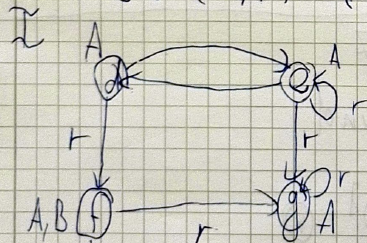
\includegraphics[width=4.71910in,height=1.83200in]{media/314typ.png}

$$t_{\MI}(d)=\{A, \exists r.A\}$$
$$t_{\MI}(e)=\{A, \exists r.A\}$$
$$t_{\MI}(f)=\{A, \exists r.A, A \sqcap B, B\}$$
$$t_{\MI}(g)=\{A, \exists r.A\}$$ \\

\begin{lemma}

Für jede Interpretation $\MI$ gilt:
$\#\left\{ t_{\MI}\left( d \right)\ |\ d \in \Delta^{\MI} \right\} \leq 2^{\left| C \right| + |T|}$
\end{lemma}

\subsubsection{Filtration}\label{filtration}

Idee:

\begin{itemize}
  \item Gegeben Interpretation $\MI$, indentifiziere alle Elemente gleichen Typs
  \item Danach kommt also jeder Typ nur einmal vor
  \item Nach Lemma 3.15 gibt es nur $2^{|C|+|\MT|}$ viele Typen
  \item Wenn $\MI$ Modell von $C$ und $\MT$, so auch das Resultat.
\end{itemize}

\begin{definition}{Filtration}

Sei $\MI$ Interpretation. Definiere Äquivalenzrelation $\sim$ auf
$\Delta^{\MI}$: $$d \sim e\ gdw.\ t_{\MI}\left( d \right) = t_{\MI}\left( e \right)$$
Wir bezeichnen diese Äquivalenzklasse von $d \in \Delta^{\MI}$ bzgl. $\sim$ mit $\left\lbrack d \right\rbrack$.

Die Filtration von $\MI$ bzgl. $C$ und $\MT$ ist folgende Interpretation $\MJ$:

\begin{itemize}
\item
  $\Delta^{\MJ} = \left\{ \left\lbrack d \right\rbrack\ |\ d \in \Delta^{\MI} \right\}$
\item
  $A^{\MJ} = \left\{ \left\lbrack d \right\rbrack\ |\ d \in A^{\MI} \right\}$
  für alle $A \in sub\left( C,\MT \right)$
\item
  $r^{\MJ} = \left\{ \left( \left\lbrack d \right\rbrack,\left\lbrack e \right\rbrack \right)|\ \exists d^{'} \in \left\lbrack d \right\rbrack,\ e^{'} \in \left\lbrack e \right\rbrack:\left( d^{'},e^{'} \right) \in r^{\MI} \right\}$
  für alle Rollennamen $r$
\end{itemize}

Beachte: $A^{\MJ}$ ist wohldefiniert (Repräsentantenunabhängigkeit)
\end{definition}

\textbf{T3.11cont}

Wenden wir diese Definition auf das Beispiel T3.11 an.

$$[d]=\{d,e,g\}$$
$$[f]=\{f\}$$

Die Interpretation $\MJ$ sieht wie folgt aus:

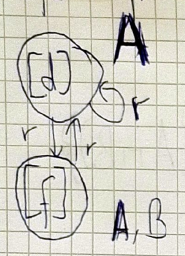
\includegraphics[width=1.21910in,height=2.33200in]{media/314typcont.png}

Offensichtlich bringt Filtration aber nicht immer das minimalste Modell, denn folgende Interpretation wäre auch ein Modell:

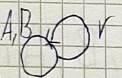
\includegraphics[width=1.0in,height=1.0in]{media/314typcont2.png}

\begin{theorem} 
Wenn $\MI$ Modell von $C$ und $\MT$, so auch $\MJ$, bzw. für alle
$d \in \Delta^{\MI}$ und $D \in sub(C,\MT)$ gilt: $d \in D^{\MI}$ gdw.
$\left\lbrack d \right\rbrack \in D^{\MJ}$.
\end{theorem}

\textbf{T3.12}

\begin{proof}
Beh.: Für alle $d \in \Delta^{\MI}$ und $D \in sub(C,\MT)$ gilt: $$d \in D^{\MI}\ gdw.\ \left\lbrack d \right\rbrack \in D^{\MJ}*$$

Beweis per Induktion über die Struktur von $D$.

\textbf{I.A.} $C = A$ * folgt aus Definition $A^{\MJ}$.

\textbf{I.S.}

\begin{enumerate}
\def\labelenumi{\arabic{enumi}.}
\item
  $\neg$, $\sqcap$ einfach mittels Semantik und I.A.
\item
  $D = \exists r.E$

  \begin{enumerate}
  \def\labelenumii{\alph{enumii}.}
  \item
    Hinrichtung

\begin{quote}
$d \in \left( \exists r.E \right)^{\MI}$ \\
$\Leftrightarrow$ (Semantik) es gibt $e \in \Delta^{\MI}$ mit $\left( d,e \right) \in r^{\MI}$ und $e \in E^{\MI}$ \\
$\Rightarrow$ (Definition $r^{\MJ}$ und I.V.) es gibt $e \in \Delta^{\MI}$ mit $\left( \left\lbrack d \right\rbrack,\left\lbrack e \right\rbrack \right) \in r^{\MJ}$ und $\left\lbrack e \right\rbrack \in E^{\MJ}$ \\
$\Leftrightarrow$ (Semantik $\exists$) $\left\lbrack d \right\rbrack \in \left( \exists r.E \right)^{\MJ}$
\end{quote}

\def\labelenumi{\alph{enumi}.}
\item
  Rückrichtung

\begin{quote}
$\left\lbrack d \right\rbrack \in \left( \exists r.E \right)^{\MJ}$ \\
$\Leftrightarrow$ (Semantik $\exists$) es gibt $[e] \in \Delta^{\MJ}$ mit $\left( \left\lbrack d \right\rbrack,\left\lbrack e \right\rbrack \right) \in r^{\MJ}$ und $\left\lbrack e \right\rbrack \in E^{\MJ}$ \\
$\Leftrightarrow$ (Definition $r^{\MJ}$ und I.V.) es gibt $[e] \in \Delta^{\MJ}$, es gibt $d^{'} \in \left\lbrack d \right\rbrack$, $e^{'} \in \left\lbrack e \right\rbrack$, $\left( d^{'},\ e^{'} \right) \in r^{\MI}$ und $e^{'} \in E^{\MI}$ \\
$\Rightarrow$ (Semantik $\exists$) $d^{'} \in \left( \exists r.E \right)^{\MI}$ \\
$\Rightarrow$ ($d \sim d^{'}$) $d \in \left( \exists r.E \right)^{\MI}$
\end{quote}

\end{enumerate}
\end{enumerate}
\end{proof}

Sei $d \in C^{\MI}$. Nach Behauptung gilt $[d] \in C^{\MJ}$, also ist $\MJ$ Modell von $C$.

$\MJ$ ist ebenfalls Modell von $\MT$:

Sei $C \sqsubseteq D$ in $\;T$, $[d] \in C^{\MJ}$ \\
Nach Beh. gilt $d \in C^{\MI}$ \\
Weil $\MI$ Modell von $C \sqsubseteq D$, gilt $d \in D^{\MI}$ \\
Nach Beh. gilt $[d] \in D^{\MJ}$

\subsubsection{Endliche/Beschränkte Modelleigenschaft}

\textbf{Theorem 3.11} \\
Wenn ein $\ALC$-Konzept $C$ bzgl. einer $\text{$\ALC$-TBox}$ $\MT$ erfüllbar ist, dann haben $C$ und $\MT$ ein gemeinsames Modell der
\emph{Kardinalität} $\leq 2^{\left| C \right| + |\MT|}$.

Beweis. Folgt aus Theorem 3.17 und Lemma 3.15.

Ähnliches (mit der selben Schranke) lässt sich für $\ALCI$ und $\ALCQ$ beweisen. (mit derselben Schranke)

\begin{theorem}
$\ALCQI$ hat nicht die endliche Modelleigenschaft.
\end{theorem}

Beweis: $A$ hat nur unendliche Modelle bzgl. folgender TBox:

\begin{itemize}
\item
  $\top \sqsubseteq \exists r.\neg A$
\item
  $T \sqsubseteq ( \leq 1\ r^{-}\ \top)$
\end{itemize}

\textbf{T3.13}

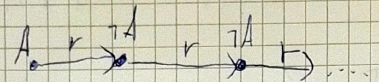
\includegraphics[width=3.21910in,height=0.93200in]{media/318qi.png}

Erklärung: Diese Interpretation müsste unendlich erweitert werden, damit es die TBox erfüllt.

\subsubsection{Entscheidbarkeit}
\textbf{Theorem 3.11}:

Wenn $C$ erfüllbar bzgl. $\MT$, dann haben $C$ und $\MT$ Modell der
Größe $\leq 2^{\left| C \right| + \left| T \right|}$.

Erfüllbarkeit ist also entscheidbar:

Gegeben $C$ und $\MT$, so dass $|C|+|\MT| = n$,
\begin{itemize} 
  \item erzeuge alle Interpretationen $\MI$ mit $\left| \Delta \right|^{\MI} \leq 2^{n}$ (es gibt höchstens $2^{2^{5n}}$ viele davon) 
  \item und überprüfe, ob $\MI$ Modell von $C$ und $\MT$ ist. (in Zeit polynomiell in $\MI$, $C$, und $\MT$)
\end{itemize}

\begin{lemma}
Gegeben sei ein $\ALC$-Konzept $C$ und endliche Interpretation $\MI$. Man kann in polynomieller Zeit -- genauer in Zeit $O\left( \left| C \right| \cdot \left| \Delta^{\MI} \right| \right)$ -- die Extension $C^{\MI}$ berechnen.
\end{lemma}

Beweisskizze zu Lemma 3.19: Rekursiver Algorithmus über die Definition der Konzeptsemantik. Dessen Zeitaufwand ist $\mathcal{O}(|C| \cdot |\Delta^{\MI}|)$:

\begin{itemize}
  \item Anzahl der (rekursiven Aufruf $= |sub(C)| \leq |C|$)
  \item pro Aufruf Zeitaufwand $\mathcal{O}(|\Delta^{\MI}|)$: \\
  simple Operationen auf $\leq 2$ Teilmengen von $\Delta^{\MI}$
\end{itemize}

\begin{korollar}
Gegeben seien $C$, $\MT$ in $\ALC$ und endliche Interpretation $\MI$. Man kann in polynomieller Zeit -- genauer: in Zeit $O(\left( \left| \MT \right| + \left| C \right| \right) \cdot \left| \Delta^{\MI} \right|)$ -- entscheiden, ob $\MI$ ein Modell von $C$ und $\MT$ ist.
\end{korollar}

\begin{theorem}
In $\ALC$ ist Erfüllbarkeit bzgl. TBoxen entscheidbar.
\end{theorem}

Die Komplexität liegt aber bei 2-ExpTime: 2-exponentiell viele Interpreationen müssen geprüft werden, jede Prüfung braucht polynomielle Zeit.

Dieser Ansatz ist kaum tauglich für die Praxis.